\documentclass[11pt]{article}
\usepackage{subcaption}

\usepackage[T1]{fontenc}
\usepackage[utf8]{inputenc}
\usepackage[a4paper,margin=1in]{geometry}
\usepackage{amsmath,amssymb}
\usepackage{booktabs}
\usepackage{array}
\usepackage{multirow}
\usepackage{hyperref}
\usepackage{graphicx}
\usepackage{xcolor}
\usepackage{graphicx}
\usepackage{tikz}
\usepackage{pgfplots}

\pgfplotsset{compat=1.18}
\usetikzlibrary{positioning}

\hypersetup{
    colorlinks=true,
    linkcolor=blue,
    citecolor=blue,
    urlcolor=blue
}

% Define custom colors to match the analysis
\definecolor{lvl0}{HTML}{1f77b4}
\definecolor{lvl1}{HTML}{ff7f0e}
\definecolor{lvl2}{HTML}{2ca02c}
\definecolor{lvl3}{HTML}{d62728}

\title{Hardware-Efficient Ansatz Design and Noise-Aware Analysis of a Variational Quantum Classifier for IQM Spark}

\author{
\begin{tabular}{c}
Iwo Wojtakajtis\textsuperscript{*}, Maria P{\l}atek\textsuperscript{*}, Rafa{\l} Balicki\textsuperscript{*}\\
Micha{\l} Szcz{\k{e}}sny\textsuperscript{*}, Karina Le{\'s}kiewicz\textsuperscript{*}, Tomasz Kajdanowicz\\[0.5em]
\small Department of Artificial Intelligence, Wroc{\l}aw University of Science and Technology, Wroc{\l}aw, Poland\\
\small Student Research Group Axion
\end{tabular}
}

\date{\today}

\begin{document}

\maketitle

\begin{abstract}
While hardware-efficient ansätze have been introduced in quantum machine learning (QML), a critical gap remains regarding the systematization and documentation of design intuitions, coupled with a lack of concrete empirical testing and evaluation on physical quantum processing units (QPUs). Consequently, there is a need to demonstrate concrete methods for evaluating  ansätze design. Standard, hardware-agnostic models still dominate the literature, often incurring massive transpilation overheads that severely degrade circuit fidelity. In this empirical study, we demonstrate that to effectively mitigate these overheads, ansatz design should be strictly tailored to the native gate set of the target device.

We present a comprehensive comparison on the binary classification benchmark, evaluating a simulator-oriented ansatz against a hardware-aligned variant tailored to the native entanglers of the IQM Spark. Moving beyond simple training accuracy, our framework evaluates five complementary dimensions: (1) compiled resource costs (2) estimated fidelity proxies; (3) theoretical expressibility via Kullback-Leibler divergence to the Haar distribution; (4) optimization robustness via five-fold cross-validation under a phenomenological expectation-value noise model; and (5) end-to-end classification performance directly on the physical QPU using Accuracy and F1 Metrics. 

Our evaluation reveals that the hardware-aligned ansatz reduces compiled circuit depth by 60\%, requiring only 19 native entanglers versus 26 in the simulator-oriented baseline. This translates to superior end-to-end classification performance on the physical IQM Spark QPU, where the tailored model achieves 82.9\% accuracy (F1: 0.783), outperforming the standard approach's 75.7\% (F1: 0.640). The physical performance advantage is underpinned by higher estimated fidelity proxies (77.90\% vs. 65.68\%). KL-divergence to the Haar pairwise-fidelity law (Section~2) shows a depth-dependent ordering: at nominal depth~2 the simulator-oriented ansatz attains lower $D_{\mathrm{KL}}$ ($0.068663$) than the hardware-aligned variant ($0.096967$), whereas at depth~4 the ordering reverses ($0.000893$ vs.\ $0.002184$); at depths $6$--$8$ both families yield small $D_{\mathrm{KL}}$ under our histogram discretization. These contrasts do not mirror the physical-QPU accuracy gap.

Our results establish hardware-native co-design as a strategic necessity rather than a theoretical compromise. While hardware-efficient models remain competitive in simulation, they demonstrate clear superiority on physical hardware. We release out five-dimensional evaluation framework as a reproducible methodology for benchmarking QML ansätze on near-term QPUs.

\end{abstract}

\noindent\textbf{Keywords:} variational quantum classifier, hardware-efficient ansatz, IQM Spark, ODRA 5, ansatz design, expressibility, cross-validation, noise-aware training

\section{Introduction}

Variational quantum classifiers (VQCs) are a prominent quantum machine learning (QML) approach for the Noisy Intermediate-Scale Quantum (NISQ) era, but their practical performance depends not only on model expressibility, but also on how efficiently the underlying circuits can be executed on physical hardware. In particular, ansätze that perform well in simulator-oriented settings may become substantially more costly after transpilation to a device-specific native gate set and coupling map, leading to increased circuit depth, higher two-qubit gate counts, and greater noise exposure.

A common strategy for mitigating this problem is to use hardware-efficient ansätze, i.e., variational circuit structures designed to remain expressive while keeping the number of parameters and the execution cost manageable under native hardware constraints~\cite{ma2024hea}. In practice, this means favoring circuit layouts compatible with the native gate set and connectivity of the target processor, rather than relying on hardware-agnostic constructions that may incur large hidden compilation overheads. This perspective motivates evaluating ansätze not only through simulator-level accuracy, but also through hardware-relevant metrics.

In this work, we study this question on the IQM Spark platform~\cite{iqmspark}, where native-gate constraints and limited qubit connectivity make transpilation overhead a practically important factor. Our experiments are conducted on ODRA~5, a five-qubit processor implementing the IQM Spark architecture, which we treat as a concrete experimental instance of this broader hardware setting.

The main contributions of this work are as follows. First, we compare a simulator-oriented variational ansatz based on parametrized controlled rotations with a hardware-aligned alternative tailored to the native entangling structure of IQM Spark. Second, we evaluate both ansatz families using a multi-dimensional framework that includes transpiled circuit cost, estimated fidelity proxies, expressibility, noise-aware optimization robustness, and end-to-end classification performance on physical hardware. Third, we show that, in this setting, a hardware-aligned design provides a practical advantage over a conventional simulator-oriented construction.

The remainder of this paper is organized as follows. Section~2 presents the theoretical framework, experimental setup, and ansatz constructions. Section~3 reports the comparative results. Section~4 discusses their implications for ansatz design in near-term QML. Sections~5 and~6 outline the limitations of the present study and provide concluding remarks.

\section{Methodology}
\subsection{Theoretical framework}
\subsubsection{Fidelity estimation}
To evaluate the impact of the hardware-native design on the performance of Variational Quantum Classifiers (VQC), we utilise an Estimated Fidelity Proxy $\mathcal{F}_{est}$. To objectively predict it, we use specific calibration data from IQM SPARK - a snapshot of the QPU's state at the exact time of execution. In the study, we base our results on the median from 10 different executions. The total fidelity is modelled as the product of independent error probabilities:$$\mathcal{F}_{est} = \mathcal{F}_{1q} \cdot \mathcal{F}_{2q} \cdot \mathcal{F}_{meas}$$Where the individual components are derived as follows:

$\mathcal{F}_{1q}$: The cumulative probability of error-free single-qubit rotations, calculated as $\prod_{i} (1 - e_{1q, i})^{n_i}$, where $e_{1q, i}$ is the error rate of the $i$-th physical qubit and $n_i$ is the number of native gates executed on it.

$\mathcal{F}_{2q}$: The probability of error-free entanglement, $\prod_{j} (1 - e_{CZ, j})^{m_j}$, where $e_{CZ, j}$ represents the error of the $j$-th physical coupling (e.g., $q_2$-$q_0$, $q_2$-$q_3$) and $m_j$ is the count of $CZ$ gates on that specific pair.

$\mathcal{F}_{meas}$: To establish a lower bound for output reliability, we incorporate a single measurement fidelity factor ($1 - e_{meas}$), representing the baseline readout error encountered by the classical observer.

The specific parameters utilized for our evaluation, reflecting the median hardware state across the experimental window, are detailed in Table 1 in Results section.




\subsubsection{Expressibility via Kullback--Leibler divergence to the Haar fidelity law}
Moment-based expressibility~\cite{sim2019} compares low-order moments of state features to their Haar averages. In parallel, we assess how closely the \emph{distribution} of a pairwise fidelity random variable---under random circuit parameters---matches the corresponding Haar law. We apply this diagnostic to the same five-qubit register as in our experiments ($D=2^{5}$), comparing the hardware-aligned ansatz and the simulator-oriented baseline at several nominal depths.

For each ansatz family, let $|\psi(\boldsymbol{\theta})\rangle$ denote the pure state prepared from a fixed initial ket. We draw independent parameter vectors $\boldsymbol{\theta}_{a}$ and $\boldsymbol{\theta}_{b}$ with i.i.d.\ coordinates uniform on $[0,2\pi)$ and define
\begin{equation}
\label{eq:pairwise-fidelity-f}
F \;=\; \bigl|\langle \psi(\boldsymbol{\theta}_{a}) | \psi(\boldsymbol{\theta}_{b}) \rangle \bigr|^{2} \in [0,1].
\end{equation}
Monte Carlo repetition yields a large sample $\{F^{(k)}\}$ for each ansatz and depth; its normalized histogram estimates the law induced by~\eqref{eq:pairwise-fidelity-f}.

For independent Haar-random pure states $|\phi_{1}\rangle,|\phi_{2}\rangle \in \mathbb{C}^{D}$, the squared overlap $|\langle \phi_{1} | \phi_{2} \rangle|^{2}$ has probability density~\cite{zyczkowski2005}
\begin{equation}
\label{eq:haar-fidelity-pdf}
p_{\mathrm{Haar}}(F) \;=\; (D-1)\,(1-F)^{D-2}, \qquad 0 \le F \le 1,
\end{equation}
the fidelity law for Haar-random states under the natural measure on pure states (equivalently, $F \sim \mathrm{Beta}(1,D-1)$).

To compare the empirical histogram to~\eqref{eq:haar-fidelity-pdf} on a \emph{common} support, we partition $[0,1]$ into $B$ equal-width bins of width $\Delta F = 1/B$. Let $p_{i}$ be the empirical bin probabilities ($\sum_{i} p_{i}=1$). For the reference we set $q_{i} \propto p_{\mathrm{Haar}}(m_{i})\,\Delta F$ with $m_{i}$ the bin midpoint, then normalize so $\sum_{i} q_{i}=1$. The reported score is the discrete Kullback--Leibler divergence (natural logarithm),
\begin{equation}
\label{eq:kl-haar-fidelity}
D_{\mathrm{KL}}(p\,\|\,q) \;=\; \sum_{i=1}^{B} p_{i}\,\ln\frac{p_{i}}{q_{i}},
\end{equation}
evaluated after small additive smoothing of both $(p_{i})$ and $(q_{i})$ so that $\ln(q_{i})$ is well defined when bins are nearly empty. Thus $D_{\mathrm{KL}}(p\,\|\,q)$ measures mismatch between the \emph{binned} empirical law and the \emph{binned} Haar reference; it approximates continuum-level KL only in the limit of fine binning and large sample size. Smaller values indicate closer agreement. The ordering $(p\,\|\,q)$ is fixed (empirical ansatz vs.\ Haar reference) and is not interchangeable: $D_{\mathrm{KL}}(q\,\|\,p)$ is a different functional.

This diagnostic is \emph{random-parameter} expressibility under uniform $\boldsymbol{\theta}$: it does \emph{not} assert that i.i.d.\ uniform gate angles induce Haar measure on the unitary group. All states are simulated as pure via exact statevector methods.

\subsubsection{Phenomenological noise modeling}

To evaluate the optimization robustness of our Variational Quantum Classifier (VQC) under realistic hardware imperfections without incurring the prohibitive computational overhead of full density-matrix simulations, we employ a phenomenological expectation-value noise model. Adapted from the framework proposed by Zhu \textit{et al.} for Quantum Graph Neural Networks\cite{Zhu2026}, this model abstracts the cumulative effect of gate infidelities and measurement errors directly into the expectation value of the observable.

Specifically, the noisy expectation value $f_{\text{noisy}}$ obtained during the evaluation of the parameterized quantum circuit is modeled as a damped and fluctuating observation:
\begin{equation}
    f_{\text{noisy}} = (1 - p_{\text{error}}) f_{\text{noiseless}} + \xi,
\end{equation}
where $f_{\text{noiseless}}$ represents the ideal, noiseless expectation value. The term $p_{\text{error}}$ defines the cumulative error probability, which scales exponentially with the circuit complexity to mimic global depolarizing effects:
\begin{equation}
    p_{\text{error}} = 1 - (1 - \epsilon)^{N_g \cdot L}.
\end{equation}
Here, $\epsilon$ refect the average per-gate error rate, $N_g$ represents the effective gate count (specifically targeting the error-prone two-qubit entanglers), and $L$ is the logical circuit depth. To simulate the inherent stochasticity of quantum measurements and unstructured device fluctuations, the additive term $\xi$ is sampled from a zero-mean Gaussian distribution:
\begin{equation}
    \xi \sim \mathcal{N}(0, \sigma_{\text{noise}}^2), \quad \text{with} \quad \sigma_{\text{noise}} = 0.2 \cdot p_{\text{error}}.
\end{equation}

This phenomenological noise layer was integrated into 5-fold cross-validation pipeline. During the classical optimization loop, gradients and cost functions were evaluated utilizing the noisy objective function $f_{\text{noisy}}$. This approach actively penalizes ans\"atze with excessive gate counts ($N_g$) and depth ($L$), allowing us to benchmark the true resilience of the parameter convergence landscape in a near-term noise regime.

\subsection{Experimental setup}
\subsubsection{Dataset and preprocessing}

We evaluate our models on the UCI Banknote Authentication dataset \cite{ucibanknote}, a binary classification benchmark comprising 1,372 samples. While the dataset does not offer an inherent quantum advantage, it was selected for its high data quality. The original data contains four continuous features extracted from wavelet-transformed images of genuine and forged banknotes. To fully utilize the 5-qubit register dictated by the target ODRA 5 hardware topology, we augment the feature space with a fifth engineered interaction term:

\begin{equation}
x_5 = x_{\mathrm{variance}} \cdot x_{\mathrm{skewness}}
\end{equation}


To map the classical data into the quantum state space, the continuous features are scaled to the interval $[-\pi/4,\pi/4]$ using min-max normalization. To map the classical data into the quantum state space, the continuous features are scaled to the interval $[-\pi/4,\pi/4]$ using min-max normalization. This restricted range is chosen to limit excessive angle magnitudes and keep the angle-encoding feature map in a controlled regime. Similarly, binary targets are remapped from $\{0,1\}$ to $\{-1,+1\}$ to naturally align with the eigenvalues of the Pauli-$Z$ observable used for measurement. No class rebalancing was applied.



\subsubsection{Execution enviroments and transpilation}


\textbf{Ideal Simulation via Qiskit Estimator}

Baseline expectation values are computed using the Qiskit StatevectorEstimator primitive. Specifically, the model's prediction for a given classical input $\mathbf{x}$ is evaluatied as: 

\begin{equation}
\langle \psi(\mathbf{x}, \boldsymbol{\theta}) | \hat{O} | \psi(\mathbf{x}, \boldsymbol{\theta}) \rangle, 
\end{equation}

where $\hat{O} = I^{\otimes 4} \otimes Z$ is a single-qubit Pauli-$Z$ observable acting on the readout qubit ($q_0$).
To integrate this quantum forward pass into our pipeline, the Estimator is wrapped inside an \texttt{EstimatorQNN} and bridged to PyTorch via a \texttt{TorchConnector}, following the Qiskit Machine Learning framework~\cite{qiskitml2025}. This hybrid setup enables gradient-based optimization, where quantum gradients are evaluated analytically using the parameter-shift rule~\cite{schuld2019grad}.

\textbf{IQM Spark ODRA 5}

Our empirical hardware evaluations are conducted on the ODRA 5, a 5-qubit superconducting quantum processing unit based on the IQM Spark architecture, hosted at the Wrocław University of Science and Technology. The physical coupling map forms an undirected star graph in which a single central qubit (\(q_2\)) is connected to each of the four peripheral qubits (\(q_0, q_1, q_3, q_4\)); no direct links exist among the peripheral qubits themselves (Fig. X).

A \textbf{native gate} is an operation that the control electronics can execute directly as a single calibrated microwave pulse, without further decomposition. The native instruction set of IQM Spark comprises parameterized single-qubit phased rotations \(R(\theta, \varphi)\) and two-qubit Controlled-\(Z\) (CZ) gates. Any logical gate outside this set or any two-qubit operation between non-adjacent qubits must be decomposed into a sequence of native instructions, increasing both circuit depth and cumulative gate error. 

\textbf{Transpilation}

The Qiskit pipeline handles gate decomposition, qubit mapping, and SWAP insertion. This study benchmarks overhead across optimization levels 0–3, though it is important to note that Levels 2 and 3 are highly sensitive to transient hardware states and daily calibration data.

Levels 0, 1: Reveal how each ansatz naturally aligns with the IQM Spark star topology through near-deterministic mapping. Level 0 establishes a naive worst-case baseline, while Level 1 uses SABRE routing~\cite{sabre2019} for a realistic cost estimate.

Levels 2, 3: Employ aggressive heuristics that maximize optimization but are significantly influenced by the specific "computer" state and calibration metrics at the time of execution

\subsubsection{Ansatz design}
The VQC pipeline utilizes independent single-qubit $R_Y(x_i)$ rotations (which compile natively to single $R$ gates) to embed the five-dimensional data into the initial quantum state. An angle-encoding strategy is used to minimize state-preparation overhead. To systematically evaluate the impact of hardware alignment, we compare two ansatz families that share a common topological macro-layer structure but differ fundamentally in their two-qubit entangling strategies.

Both ansätze are constructed from $m = \lfloor L/2 \rfloor$ repeating macro-layers, where $L \in \{2, 4, 6\}$ denotes the nominal circuit depth. Each macro-layer comprises four sequential sub-layers: 
(1) single-qubit $R_Y$ rotations applied to all qubits; 
(2) parameterized forward entanglement along a logical ring connectivity, contributing one trainable parameter per edge, coupling qubit $i$ to $(i+1) \bmod n$; 
(3) single-qubit $R_X$ rotations on all qubits; and 
(4) parameterized reverse entanglement along the ring, similarly contributing one parameter per edge, coupling $i$ to $(i-1) \bmod n$. 

This bidirectional logical connectivity ensures that correlations propagate rapidly in both directions across the 5-qubit register. To optimize efficiency, the reverse entanglement sub-layer in the final macro-layer is trimmed to include only the edges directly incident on the readout qubit ($q_0$). Because the final classification decision relies solely on a Pauli-$Z$ observable measured on $q_0$, this trimming prunes operations that would otherwise contribute to cumulative gate error without fundamentally altering the causal lightcone of the measurement. Consequently, this architecture yields $(m-1) \cdot 4n + (3n+2)$ trainable parameters—scaling from 17 parameters at $L=2$ up to 57 parameters at $L=6$.

\textbf{Simulator-Oriented Ansatz.} The baseline simulation variant \cite{havlicek2019} utilizes fully parameterized controlled rotations: $CR_X(\theta)$ for the forward pass and $CR_Y(\theta)$ for the reverse pass. These gates serve as a standard textbook choice for generating parameterized entanglement in idealized VQC research. However, transpiling these continuous entanglers to an IQM Spark native instruction set is prohibitively expensive. At raw transpilation (optimization level 0), a single $CR_X$ gate decomposes into 16 native $R$ gates and 2 $CZ$ gates (circuit depth 18), while a $CR_Y$ gate requires 10 $R$ gates and 2 $CZ$ gates (depth 12).

\textbf{Hardware-Aligned (ODRA) Ansatz.}
To reduce overhead, the ODRA ansatz~\cite{abbas2021} substitutes controlled rotations with hardware-native $CZ$ gates preceded by $R_Z(\theta)$ or $R_Y(\theta)$ rotations for the forward and reverse sub-layers, respectively. Although this is not mathematically equivalent to a controlled rotations, these single-qubit rotations parameterize the local state basis prior to interaction. This yields a comparable variational family that explores the Hilbert space while mapping directly to single-pulse native hardware execution, reducing both transpiled depth and cumulative error.

\subsubsection{Depth and gate count}

To quantify the structural efficiency of the proposed architectures, we evaluate circuit complexity across the three previously defined nominal depths ($L \in \{2, 4, 6\}$). To provide a rigorous empirical comparison between logical design and physical implementation, we define two distinct comparative metrics:
\begin{itemize}
    \item \textbf{Logical Depth:} The number of abstract entangling layers in the idealized model prior to transpilation.
    \item \textbf{Physical Depth:} The total number of sequential pulse layers required after the circuit has been fully mapped to the hardware's native topology and instruction set.
\end{itemize}
We further categorize compiled operations into native $N_{1q}$ and $N_{2q}$ gates. By tracking the inflation of compiled $N_{2q}$ counts alongside Physical Depth, we demonstrate the severe overhead gap incurred by simulator-oriented ansätze compared to their hardware-tailored counterparts.

\subsubsection{Odra bUUUUUst}



\section{Results}

\subsection{Fidelity}
VQC fidelity was calculated using daily IQM SPARK calibration data averaged over the 5-day experimental window, with the hardware parameters detailed in Table \ref{tab:calibration_metrics}. The hardware remained stable throughout, with an average standard deviation of 0.001127948 (max: 0.003518181). This methodology provides a realistic error budget by quantifying how circuit complexity directly impacts performance, enabling a rigorous comparison of algorithmic robustness. As shown in Table \ref{tab:fidelity_results}, the hardware-efficient \texttt{ansatz\_odra} achieves significantly higher fidelity than the \texttt{ansatz\_simulator} baseline across all configurations, confirming the clear advantage of hardware-native design in mitigating noise.

\begin{table}[htbp]
\centering
\caption{Average Calibration Metrics for the IQM SPARK QPU (Star Topology).}
\label{tab:calibration_metrics}
\begin{tabular}{llcc}
\toprule
\textbf{Component} & \textbf{Type} & \textbf{Error Rate ($e$)} & \textbf{Fidelity ($1-e$)} \\
\midrule
Qubit $q_1$ (Spoke) & Single-qubit & 0.128\% & 0.99872 \\
Qubit $q_2$ (Spoke) & Single-qubit & 0.112\% & 0.99888 \\
Qubit $q_3$ (Hub)   & Single-qubit & 0.098\% & 0.99902 \\
Qubit $q_4$ (Spoke) & Single-qubit & 0.110\% & 0.99890 \\
Qubit $q_5$ (Spoke) & Single-qubit & 0.134\% & 0.99866 \\
\midrule
Coupling $q_3 \leftrightarrow q_1$ & Two-qubit (CZ) & 0.836\% & 0.99164 \\
Coupling $q_3 \leftrightarrow q_2$ & Two-qubit (CZ) & 0.792\% & 0.99208 \\
Coupling $q_3 \leftrightarrow q_4$ & Two-qubit (CZ) & 1.040\% & 0.98960 \\
Coupling $q_3 \leftrightarrow  w2`                                           q_5$ & Two-qubit (CZ) & 1.172\% & 0.98828 \\
\midrule
Qubit $q_1$ & Measurement & 1.780\% & 0.98220 \\
\bottomrule
\end{tabular}
\end{table}

To visualize these scaling trends and the relative performance advantage, the following figures illustrate the absolute fidelity and the resulting fidelity gap across all tested circuit depths and optimization levels.

\begin{figure}[htbp]
    \centering
    % --- LEFT: FIDELITY ---
    \begin{subfigure}[b]{0.49\textwidth}
        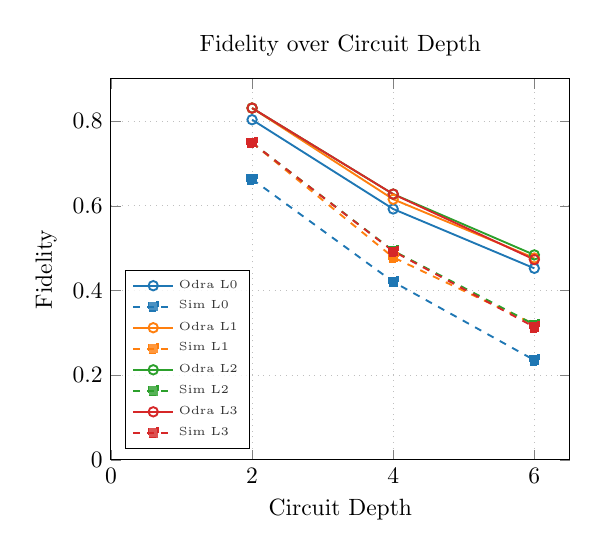
\begin{tikzpicture}[scale=0.85]
        \begin{axis}[
            title={Fidelity over Circuit Depth},
            xlabel={Circuit Depth},
            ylabel={Fidelity},
            xmin=0, xmax=6.5,
            ymin=0, ymax=0.9,
            xtick={0,2,4,6},
            scaled y ticks=false, % Wyłącza notację naukową
            yticklabel style={
                /pgf/number format/fixed,
                /pgf/number format/precision=2
            },
            grid=major,
            grid style={dotted,gray!50},
            % Legend moved inside to the bottom-left
            legend style={at={(0.03,0.03)}, anchor=south west, font=\tiny, cells={anchor=west}, fill opacity=0.8, draw opacity=1}
        ]
            % Level 0
            \addplot[color=lvl0, mark=o, thick] coordinates {(2,0.8035) (4,0.5926) (6,0.4525)};
            \addplot[color=lvl0, mark=square*, dashed, thick] coordinates {(2,0.6631) (4,0.4206) (6,0.2357)};
            
            % Level 1
            \addplot[color=lvl1, mark=o, thick] coordinates {(2,0.8310) (4,0.6156) (6,0.4769)};
            \addplot[color=lvl1, mark=square*, dashed, thick] coordinates {(2,0.7490) (4,0.4784) (6,0.3203)};

            % Level 2
            \addplot[color=lvl2, mark=o, thick] coordinates {(2,0.8310) (4,0.6278) (6,0.4842)};
            \addplot[color=lvl2, mark=square*, dashed, thick] coordinates {(2,0.7490) (4,0.4940) (6,0.3195)};

            % Level 3
            \addplot[color=lvl3, mark=o, thick] coordinates {(2,0.8310) (4,0.6278) (6,0.4732)};
            \addplot[color=lvl3, mark=square*, dashed, thick] coordinates {(2,0.7490) (4,0.4929) (6,0.3139)};

            \legend{Odra L0, Sim L0, Odra L1, Sim L1, Odra L2, Sim L2, Odra L3, Sim L3}
        \end{axis}
        \end{tikzpicture}
    \end{subfigure}
    \hfill
    % --- RIGHT: FIDELITY GAP ---
    \begin{subfigure}[b]{0.49\textwidth}
        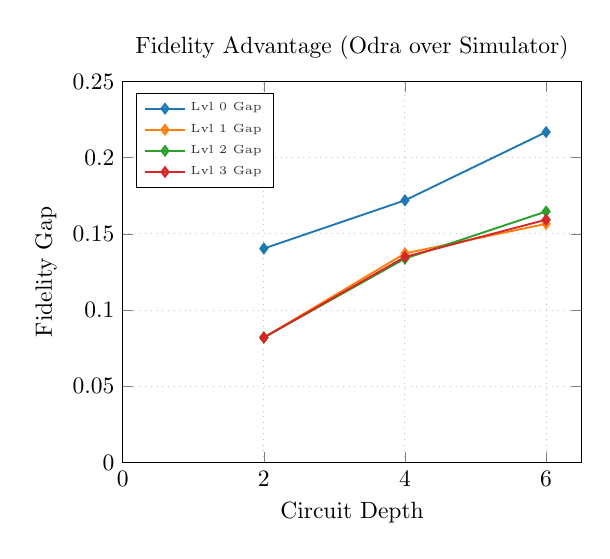
\begin{tikzpicture}[scale=0.85]
        \begin{axis}[
            title={Fidelity Advantage (Odra over Simulator)},
            xlabel={Circuit Depth},
            ylabel={Fidelity Gap},
            xmin=0, xmax=6.5,
            ymin=0, ymax=0.25,
            xtick={0,2,4,6},
            scaled y ticks=false, % Wyłącza notację naukową (5 * 10^-2)
            yticklabel style={
                /pgf/number format/fixed, % Wymusza zapis dziesiętny (0.05)
                /pgf/number format/precision=2
            },
            grid=major,
            grid style={dotted,gray!50},
            % Legend moved inside to the top-left
            legend style={at={(0.03,0.97)}, anchor=north west, font=\tiny, fill opacity=0.8, draw opacity=1}
        ]
            \addplot[color=lvl0, mark=diamond*, thick] coordinates {(2,0.1404) (4,0.1720) (6,0.2168)};
            \addplot[color=lvl1, mark=diamond*, thick] coordinates {(2,0.0820) (4,0.1372) (6,0.1566)};
            \addplot[color=lvl2, mark=diamond*, thick] coordinates {(2,0.0820) (4,0.1338) (6,0.1647)};
            \addplot[color=lvl3, mark=diamond*, thick] coordinates {(2,0.0820) (4,0.1349) (6,0.1593)};

            \legend{Lvl 0 Gap, Lvl 1 Gap, Lvl 2 Gap, Lvl 3 Gap}
        \end{axis}
        \end{tikzpicture}
    \end{subfigure}
    \caption{Comparative analysis of circuit fidelity.}
    \label{fig:fidelity_internal_legends}
\end{figure}

These results reveal a critical divergence in scalability. While the \texttt{ansatz\_simulator} drops below the 50\% fidelity threshold by depth 4 - entering a noise-dominated regime where outputs become statistically unreliable - the \texttt{ansatz\_odra} maintains a much higher success probability. The fact that the performance gap between them widens as the circuit grows demonstrates that hardware-native design is not merely a preference, but a fundamental requirement for preserving computational utility as quantum algorithms scale.


\subsection{Expressibility}

Table~\ref{tab:kl_haar} reports the discrete divergence $D_{\mathrm{KL}}(p_{\mathrm{emp}}\,\|\,q_{\mathrm{Haar}})$ defined in~\eqref{eq:kl-haar-fidelity}, evaluated under the sampling scheme and Haar reference of Section~2 with $B=150$ bins and $10^{5}$ Monte Carlo draws per ansatz and nominal depth. Figure~\ref{fig:kl_haar_depth} plots the same estimates on a logarithmic vertical scale.

\begin{table}[htbp]
    \centering
    \caption{Haar pairwise-fidelity law diagnostic: $D_{\mathrm{KL}}(p_{\mathrm{emp}}\,\|\,q_{\mathrm{Haar}})$ for \texttt{ansatz\_odra} (hardware-aligned) and \texttt{ansatz\_simulator} (simulator-oriented). The final column identifies which ansatz attains the smaller divergence at each depth (i.e.\ closer agreement with the binned reference under~\eqref{eq:kl-haar-fidelity}).}
    \label{tab:kl_haar}
    \renewcommand{\arraystretch}{1.15}
    \begin{tabular}{c r r l}
        \toprule
        \textbf{Nominal depth} & \textbf{ODRA} & \textbf{Simulator} & \textbf{Smaller $D_{\mathrm{KL}}$} \\
        \midrule
        2 & $0.096967$ & $0.068663$ & Simulator \\
        4 & $0.000893$ & $0.002184$ & ODRA \\
        6 & $0.000256$ & $0.000323$ & ODRA \\
        8 & $0.000298$ & $0.000240$ & Simulator \\
        \bottomrule
    \end{tabular}
\end{table}

\begin{figure}[htbp]
    \centering
    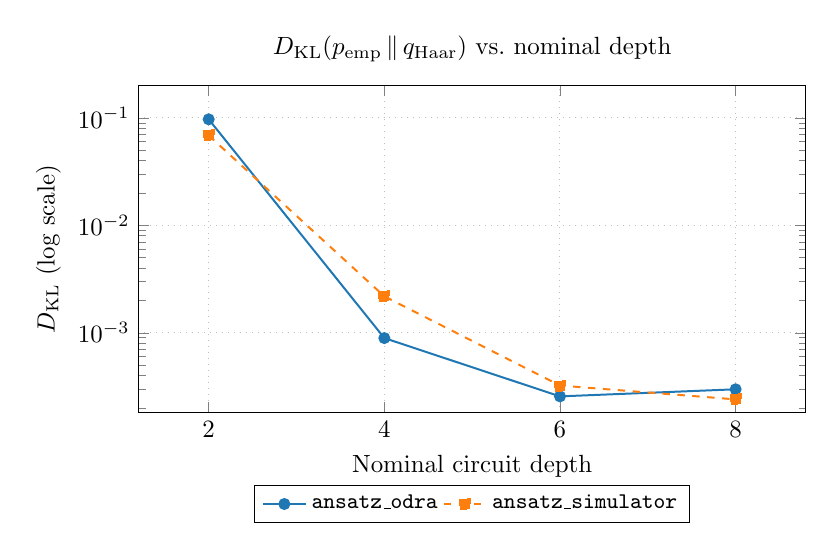
\begin{tikzpicture}[scale=0.9]
        \begin{axis}[
            width=11cm,
            height=6.2cm,
            ymode=log,
            title={$D_{\mathrm{KL}}(p_{\mathrm{emp}}\,\|\,q_{\mathrm{Haar}})$ vs.\ nominal depth},
            xlabel={Nominal circuit depth},
            ylabel={$D_{\mathrm{KL}}$ (log scale)},
            xmin=1.2, xmax=8.8,
            ymin=1.8e-4, ymax=0.2,
            xtick={2,4,6,8},
            scaled y ticks=false,
            grid=major,
            grid style={dotted,gray!50},
            legend style={at={(0.5,-0.22)}, anchor=north, legend columns=2, font=\small},
        ]
            \addplot[color=lvl0, mark=*, thick] coordinates {(2,0.096967) (4,0.000893) (6,0.000256) (8,0.000298)};
            \addplot[color=lvl1, mark=square*, dashed, thick] coordinates {(2,0.068663) (4,0.002184) (6,0.000323) (8,0.000240)};
            \legend{\texttt{ansatz\_odra}, \texttt{ansatz\_simulator}}
        \end{axis}
    \end{tikzpicture}
    \caption{Summary of Table~\ref{tab:kl_haar}. The relative ranking of the two ansätze is not monotone in depth; beyond $L=2$ both curves lie at substantially smaller $D_{\mathrm{KL}}$ than at $L=2$.}
    \label{fig:kl_haar_depth}
\end{figure}

The relative performance of the two constructions under this diagnostic is depth-dependent. The simulator-oriented ansatz yields the smaller divergence at $L=2$ and marginally at $L=8$; the hardware-aligned ansatz does so at $L\in\{4,6\}$. For $L\ge 4$, both values are small relative to $L=2$, which indicates close agreement between empirical and reference bin probabilities under the chosen histogram and sample size. These conclusions concern ideal circuits with uniformly random parameters and do not subsume data encoding, device noise, or transpilation; they are therefore best viewed as a complement to, rather than a substitute for, the hardware and training analyses reported above. Implementation details are documented in the accompanying repository~\cite{qc1repo}.

\subsection{Noise}

To evaluate the baseline optimization quality and robustness of our ans\"atze, we employed a phenomenological expectation-value noise model. Following recent literature, we applied a near-term realistic per-gate error rate of $\epsilon = 0.005$, which translates into a noise probability that scales exponentially with the effective gate count and logical circuit depth. The primary objective of this evaluation is to determine whether our ans\"atze architectures are well-fitted and properly optimized in their ideal states. According to the framework established by Zhu et al., if the introduction of noise systematically degrades performance, it confirms that the models are already highly optimized; conversely, if noise acts as an implicit regularizer and improves the classification metrics, it would indicate that the baseline models are under-optimized and trapped in suboptimal local minima.

\begin{table}[htbp]
    \centering
    \caption{5-Fold Cross-Validation Performance Metrics under Ideal and Phenomenological Noise Environments}
    \label{tab:noise_cv}
    \renewcommand{\arraystretch}{1.2}
    \begin{tabular}{llccc}
        \hline
        \textbf{Depth} & \textbf{Model} & \textbf{Environment} & \textbf{Mean Accuracy $\pm$ Std} & \textbf{Mean F1 $\pm$ Std} \\ \hline
        2 & Odra & Ideal & $0.8615 \pm 0.0203$ & $0.8301 \pm 0.0295$ \\
        2 & Odra & Noise & $0.8593 \pm 0.0181$ & $0.8245 \pm 0.0256$ \\
        2 & Simulator & Ideal & $0.8863 \pm 0.0134$ & $0.8633 \pm 0.0198$ \\
        2 & Simulator & Noise & $0.8739 \pm 0.0142$ & $0.8454 \pm 0.0226$ \\ \hline
        4 & Odra & Ideal & $0.8717 \pm 0.0233$ & $0.8423 \pm 0.0438$ \\
        4 & Odra & Noise & $0.8528 \pm 0.0289$ & $0.8111 \pm 0.0545$ \\
        4 & Simulator & Ideal & $0.8776 \pm 0.0292$ & $0.8494 \pm 0.0507$ \\
        4 & Simulator & Noise & $0.8550 \pm 0.0215$ & $0.8184 \pm 0.0411$ \\ \hline
    \end{tabular}
\end{table}

\begin{figure}[htbp]
    \centering
    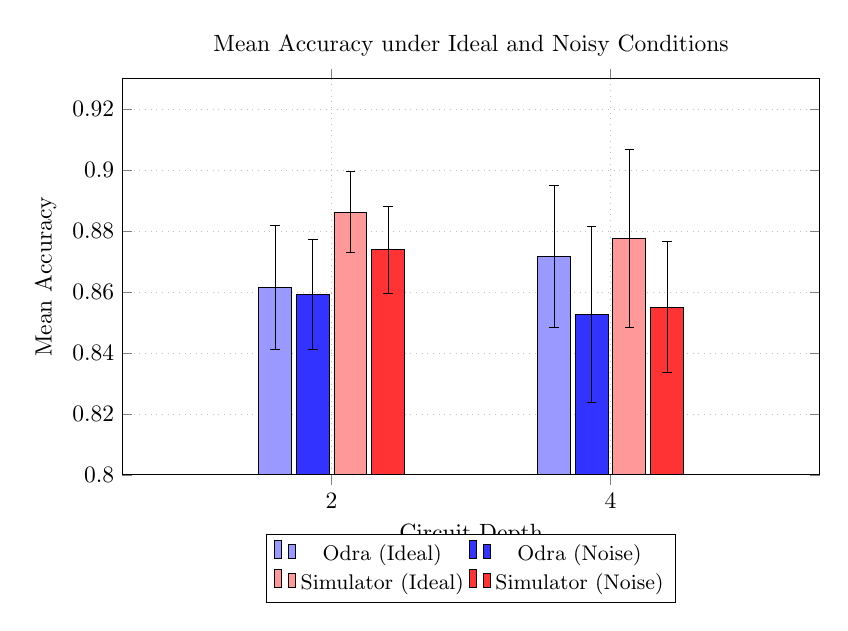
\begin{tikzpicture}[scale=0.85]
    \begin{axis}[
        ybar=2pt,
        bar width=14pt,
        width=12cm,
        height=7.5cm,
        title={Mean Accuracy under Ideal and Noisy Conditions},
        xlabel={Circuit Depth},
        ylabel={Mean Accuracy},
        xmin=0.5, xmax=5.5,
        xtick={2, 4},
        ymin=0.80, ymax=0.93,
        scaled y ticks=false,
        yticklabel style={
            /pgf/number format/fixed,
            /pgf/number format/precision=2
        },
        grid=major,
        grid style={dotted,gray!50},
        legend style={at={(0.5,-0.15)}, anchor=north, legend columns=2, font=\small},
        error bars/y dir=both,
        error bars/y explicit
    ]
        % Odra Ideal
        \addplot[fill=blue!40, draw=black] coordinates {(2,0.8615) +- (0,0.0203) (4,0.8717) +- (0,0.0233)};
        % Odra Noise
        \addplot[fill=blue!80, draw=black] coordinates {(2,0.8593) +- (0,0.0181) (4,0.8528) +- (0,0.0289)};
        % Simulator Ideal
        \addplot[fill=red!40, draw=black] coordinates {(2,0.8863) +- (0,0.0134) (4,0.8776) +- (0,0.0292)};
        % Simulator Noise
        \addplot[fill=red!80, draw=black] coordinates {(2,0.8739) +- (0,0.0142) (4,0.8550) +- (0,0.0215)};

        \legend{Odra (Ideal), Odra (Noise), Simulator (Ideal), Simulator (Noise)}
    \end{axis}
    \end{tikzpicture}
    \caption{Comparison of Mean Accuracy across Depth 2 and Depth 4 configurations. Error bars represent one standard deviation from the cross-validation.}
    \label{fig:noise_cv_chart}
\end{figure}

As detailed in Table \ref{tab:noise_cv} and Figure \ref{fig:noise_cv_chart}, the empirical data reveals a clear and universal degradation in both Mean Accuracy and F1 metrics across all our tested ans\"atze when transitioning from the noiseless regime to the noisy environment. For both depth configurations, the introduction of the noise penalty consistently suppressed classification performance and disrupted the finely tuned representations. Crucially, we observed absolutely no instances of noise-induced performance enhancement. Interpreted through the previously discussed theoretical lens, this universal decline serves as strong empirical validation that our ans\"atze are already highly optimized and well-converged in their native states. Rather than benefiting from noise as an implicit regularizer, the well-conditioned parameterizations of our models are simply destabilized by the stochastic errors. Consequently, these findings confirm the structural quality and baseline optimization of our designs, demonstrating that they successfully reach near-optimal parameterizations prior to the introduction of hardware-level noise.


\subsection{Depth and gate count}

Deep, unoptimized quantum circuits suffer from increased decoherence times and exacerbate the barren plateau problem during variational training. Because two-qubit control gates are the dominant source of noise in current NISQ architectures, minimizing compilation overhead is critical. 

\begin{figure}[htbp]
    \centering
    
    % ================= ROW 1 =================
    
    % --- GRAPH 1: Physical Depth ---
    \begin{subfigure}[b]{0.48\textwidth}
        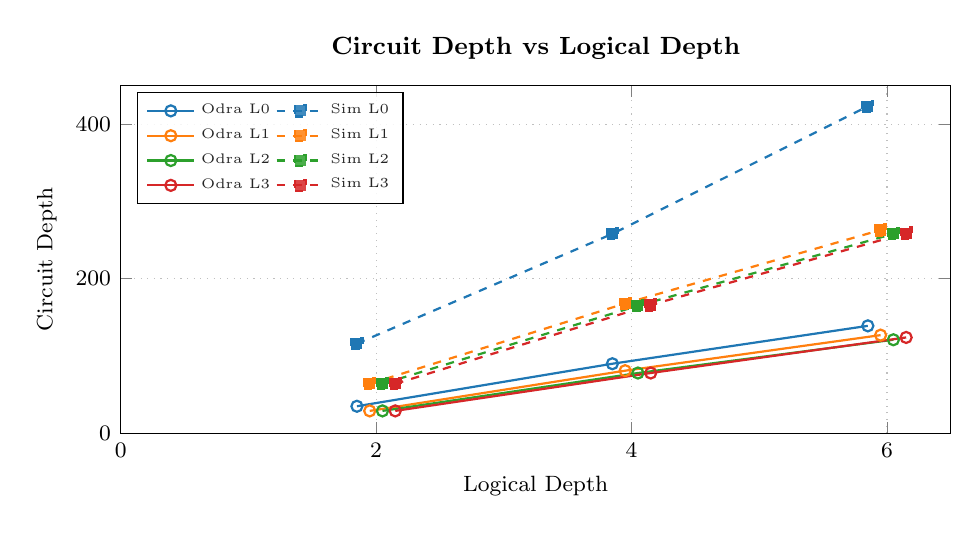
\begin{tikzpicture}
        \begin{axis}[
            width=\linewidth, height=6cm,
            title={Circuit Depth vs Logical Depth},
            xlabel={Logical Depth}, ylabel={Circuit Depth},
            xmin=0, xmax=6.5, ymin=0, ymax=450, xtick={0,2,4,6}, % <-- Zmieniono na xmin=0 i dodano 0 do xtick
            grid=major, grid style={dotted,gray!50},
            label style={font=\footnotesize}, tick label style={font=\footnotesize}, title style={font=\small\bfseries},
            legend style={at={(0.02,0.98)}, anchor=north west, legend columns=2, font=\tiny, fill opacity=0.85}
        ]
            % Level 0 (Shift -0.15)
            \addplot[color=lvl0, mark=o, thick] coordinates {(1.85,35) (3.85,90) (5.85,139)};
            \addplot[color=lvl0, mark=square*, dashed, thick] coordinates {(1.85,116) (3.85,258) (5.85,423)};
            % Level 1 (Shift -0.05)
            \addplot[color=lvl1, mark=o, thick] coordinates {(1.95,29) (3.95,81) (5.95,127)};
            \addplot[color=lvl1, mark=square*, dashed, thick] coordinates {(1.95,64) (3.95,168) (5.95,263)};
            % Level 2 (Shift +0.05)
            \addplot[color=lvl2, mark=o, thick] coordinates {(2.05,29) (4.05,78) (6.05,121)};
            \addplot[color=lvl2, mark=square*, dashed, thick] coordinates {(2.05,64) (4.05,165) (6.05,258)};
            % Level 3 (Shift +0.15)
            \addplot[color=lvl3, mark=o, thick] coordinates {(2.15,29) (4.15,78) (6.15,124)};
            \addplot[color=lvl3, mark=square*, dashed, thick] coordinates {(2.15,64) (4.15,166) (6.15,259)};
            
            \legend{Odra L0, Sim L0, Odra L1, Sim L1, Odra L2, Sim L2, Odra L3, Sim L3}
        \end{axis}
        \end{tikzpicture}
    \end{subfigure}
    \hfill
    % --- GRAPH 2: Total Gates ---
    \begin{subfigure}[b]{0.48\textwidth}
        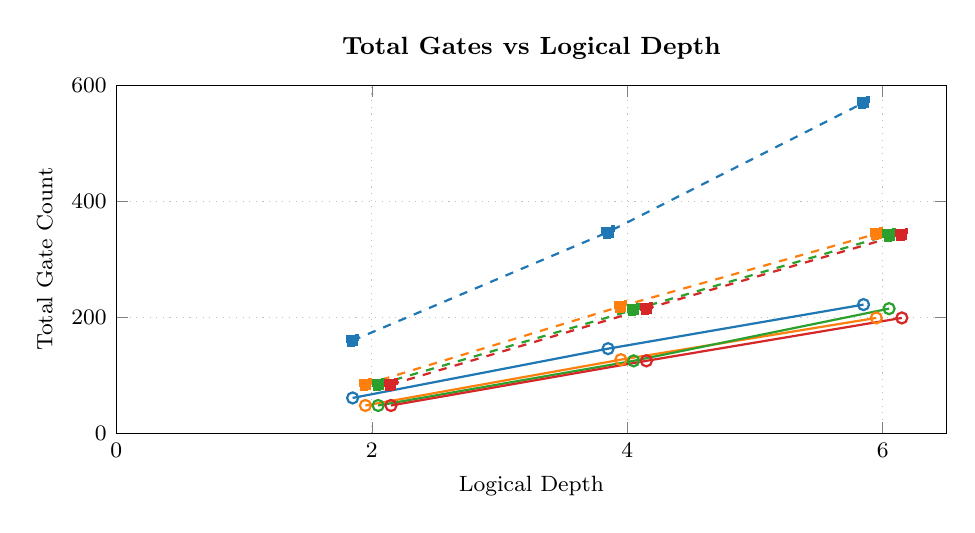
\begin{tikzpicture}
        \begin{axis}[
            width=\linewidth, height=6cm,
            title={Total Gates vs Logical Depth},
            xlabel={Logical Depth}, ylabel={Total Gate Count},
            xmin=0, xmax=6.5, ymin=0, ymax=600, xtick={0,2,4,6}, % <-- Zmieniono na xmin=0 i dodano 0 do xtick
            grid=major, grid style={dotted,gray!50},
            label style={font=\footnotesize}, tick label style={font=\footnotesize}, title style={font=\small\bfseries}
        ]
            % Level 0 (-0.15)
            \addplot[color=lvl0, mark=o, thick] coordinates {(1.85,61) (3.85,146) (5.85,222)};
            \addplot[color=lvl0, mark=square*, dashed, thick] coordinates {(1.85,160) (3.85,347) (5.85,570)};
            % Level 1 (-0.05)
            \addplot[color=lvl1, mark=o, thick] coordinates {(1.95,48) (3.95,127) (5.95,199)};
            \addplot[color=lvl1, mark=square*, dashed, thick] coordinates {(1.95,84) (3.95,219) (5.95,344)};
            % Level 2 (+0.05)
            \addplot[color=lvl2, mark=o, thick] coordinates {(2.05,48) (4.05,125) (6.05,215)};
            \addplot[color=lvl2, mark=square*, dashed, thick] coordinates {(2.05,84) (4.05,213) (6.05,342)};
            % Level 3 (+0.15)
            \addplot[color=lvl3, mark=o, thick] coordinates {(2.15,48) (4.15,125) (6.15,199)};
            \addplot[color=lvl3, mark=square*, dashed, thick] coordinates {(2.15,84) (4.15,215) (6.15,343)};
        \end{axis}
        \end{tikzpicture}
    \end{subfigure}
    
    \vspace{0.4cm}
    
    % ================= ROW 2 =================
    
    % --- GRAPH 3: Control Gates ---
    \begin{subfigure}[b]{0.48\textwidth}
        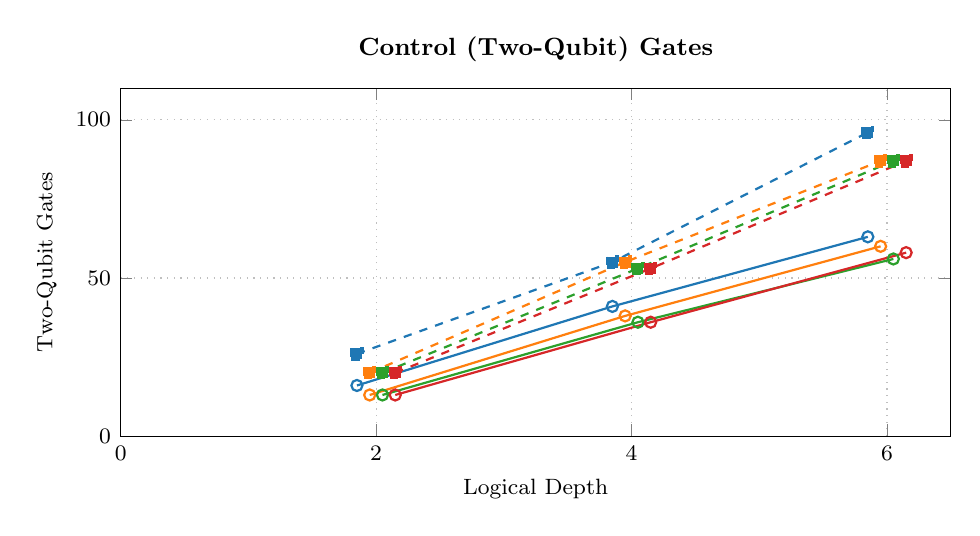
\begin{tikzpicture}
        \begin{axis}[
            width=\linewidth, height=6cm,
            title={Control (Two-Qubit) Gates},
            xlabel={Logical Depth}, ylabel={Two-Qubit Gates},
            xmin=0, xmax=6.5, ymin=0, ymax=110, xtick={0,2,4,6}, % <-- Zmieniono na xmin=0 i dodano 0 do xtick
            grid=major, grid style={dotted,gray!50},
            label style={font=\footnotesize}, tick label style={font=\footnotesize}, title style={font=\small\bfseries}
        ]
            % Level 0 (-0.15)
            \addplot[color=lvl0, mark=o, thick] coordinates {(1.85,16) (3.85,41) (5.85,63)};
            \addplot[color=lvl0, mark=square*, dashed, thick] coordinates {(1.85,26) (3.85,55) (5.85,96)};
            % Level 1 (-0.05)
            \addplot[color=lvl1, mark=o, thick] coordinates {(1.95,13) (3.95,38) (5.95,60)};
            \addplot[color=lvl1, mark=square*, dashed, thick] coordinates {(1.95,20) (3.95,55) (5.95,87)};
            % Level 2 (+0.05)
            \addplot[color=lvl2, mark=o, thick] coordinates {(2.05,13) (4.05,36) (6.05,56)};
            \addplot[color=lvl2, mark=square*, dashed, thick] coordinates {(2.05,20) (4.05,53) (6.05,87)};
            % Level 3 (+0.15)
            \addplot[color=lvl3, mark=o, thick] coordinates {(2.15,13) (4.15,36) (6.15,58)};
            \addplot[color=lvl3, mark=square*, dashed, thick] coordinates {(2.15,20) (4.15,53) (6.15,87)};
        \end{axis}
        \end{tikzpicture}
    \end{subfigure}
    \hfill
    % --- GRAPH 4: Estimator vs IQM ---
    \begin{subfigure}[b]{0.48\textwidth}
        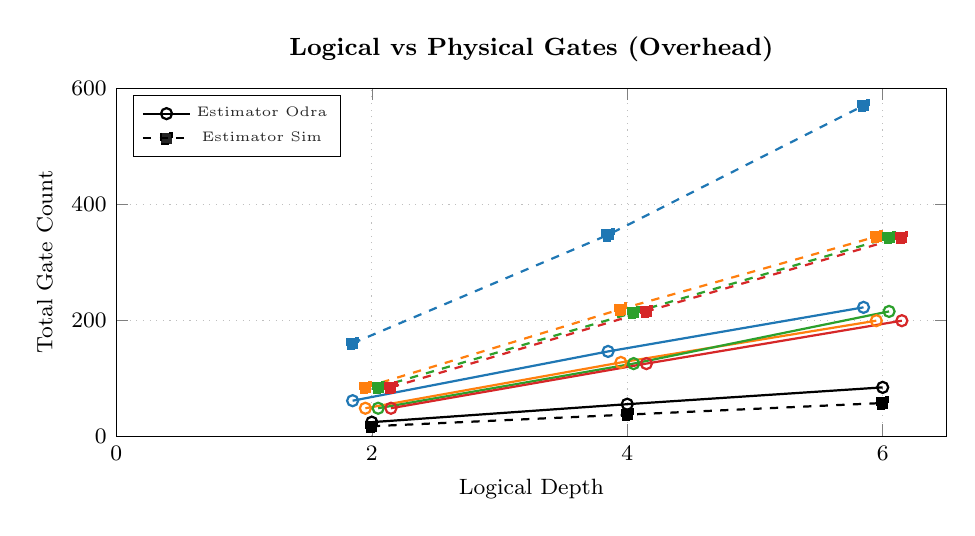
\begin{tikzpicture}
        \begin{axis}[
            width=\linewidth, height=6cm,
            title={Logical vs Physical Gates (Overhead)},
            xlabel={Logical Depth}, ylabel={Total Gate Count},
            xmin=0, xmax=6.5, ymin=0, ymax=600, xtick={0,2,4,6}, % <-- Zmieniono na xmin=0 i dodano 0 do xtick
            grid=major, grid style={dotted,gray!50},
            label style={font=\footnotesize}, tick label style={font=\footnotesize}, title style={font=\small\bfseries},
            legend style={at={(0.02,0.98)}, anchor=north west, font=\tiny, fill opacity=0.85}
        ]
            % Estimator Baseline (Ideal) - Black lines plotted first
            \addplot[color=black, mark=o, thick] coordinates {(2,24) (4,55) (6,84)};
            \addplot[color=black, mark=square*, dashed, thick] coordinates {(2,17) (4,37) (6,57)};
            
            % IQM Spark Lines (Shifted to not cover the Estimator)
            \addplot[color=lvl0, mark=o, thick] coordinates {(1.85,61) (3.85,146) (5.85,222)};
            \addplot[color=lvl0, mark=square*, dashed, thick] coordinates {(1.85,160) (3.85,347) (5.85,570)};
            \addplot[color=lvl1, mark=o, thick] coordinates {(1.95,48) (3.95,127) (5.95,199)};
            \addplot[color=lvl1, mark=square*, dashed, thick] coordinates {(1.95,84) (3.95,219) (5.95,344)};
            \addplot[color=lvl2, mark=o, thick] coordinates {(2.05,48) (4.05,125) (6.05,215)};
            \addplot[color=lvl2, mark=square*, dashed, thick] coordinates {(2.05,84) (4.05,213) (6.05,342)};
            \addplot[color=lvl3, mark=o, thick] coordinates {(2.15,48) (4.15,125) (6.15,199)};
            \addplot[color=lvl3, mark=square*, dashed, thick] coordinates {(2.15,84) (4.15,215) (6.15,343)};
            
            \legend{Estimator Odra, Estimator Sim}
        \end{axis}
        \end{tikzpicture}
    \end{subfigure}
    \caption{Hardware compilation analysis across optimization levels.}
    \label{fig:gate_overhead_grid}
\end{figure}

The structural alignment of the \texttt{ansatz\_odra} with the physical QPU topology provides a massive advantage in compilation efficiency. While the \texttt{ansatz\_simulator} appears highly efficient at the logical level (as seen in the black Estimator baseline in Graph 4), it suffers a severe transpilation penalty when mapped to physical hardware. By natively minimizing circuit depth and avoiding excessive SWAP gate insertions, hardware-aware design is essential for scaling variational algorithms effectively on restricted hardware topologies.

\subsection{bUUUUst}


\section{Discussion}

% TODO: This section is a working draft and should be refined once the remaining
% results, tables, and figures are finalized. Statements marked as
% [RESULT-DEPENDENT] should be aligned with the final quantitative trends.

The results support the view that ansatz design for near-term quantum machine learning should be treated as a hardware-aware problem rather than as a purely simulator-oriented modeling choice. In the present setting, the hardware-aligned ansatz appears to benefit from a closer match to the native execution constraints of the IQM Spark platform, indicating that practical performance depends not only on the abstract circuit structure, but also on how efficiently that structure can be implemented on physical hardware.
% [RESULT-DEPENDENT]: adjust the strength of this claim depending on the final consistency of the advantage across all reported metrics.

A key mechanism behind this behavior is transpilation overhead. The difference between the compared ansatz families is not explained solely by their logical design, but by the cost of mapping them to the native gate set and coupling map. On hardware with constrained connectivity and native entangling operations, this cost directly affects circuit depth, two-qubit gate count, and cumulative noise exposure. From this perspective, the hardware-aligned ansatz should not be viewed simply as a lighter approximation, but as a design that better preserves its intended structure under physical execution.
% [STABLE]: keep unless the transpilation analysis changes substantially.

At the same time, the present comparison suggests that theoretical expressibility is not sufficient on its own to predict end-to-end classification quality on a physical QPU. Even when expressibility differences are observed, they may become less important in practice than compiled resource costs and hardware noise. This supports a broader evaluation strategy in which simulator-level properties are interpreted together with fidelity-oriented, compilation-aware, and hardware-level metrics rather than in isolation.
% [RESULT-DEPENDENT]: revise this paragraph once the final expressibility and noise-related results are fixed.

More broadly, our findings do not imply that a more hardware-efficient ansatz is always preferable in every QML setting. Rather, they show that ansatz quality is hardware-context dependent, and that benchmarking on near-term processors should explicitly account for compilation overhead, native-gate realism, and noise sensitivity. In this sense, the main value of the present study lies not only in the comparison of two ansatz families on a single task, but also in illustrating hardware-native co-design as a practically important principle for evaluating variational models on platforms such as IQM Spark.
% [STABLE]: this paragraph can remain close to the final version.

\section{Limitations}

Several limitations should be considered when interpreting the results of this study. First, the empirical analysis is conducted in a five-qubit regime on a specific instance of the IQM Spark architecture. While this setting is sufficient to expose the practical consequences of transpilation overhead, native-gate constraints, and limited connectivity, it does not by itself establish that the same quantitative trends will persist for larger registers or for architectures with different coupling maps and calibration profiles.

Second, our experimental benchmark is restricted to a single binary classification task based on the UCI Banknote Authentication dataset. Although this dataset provides a convenient and reproducible testbed for comparing ansatz families, it represents only one learning scenario with a low-dimensional feature space. As a result, the present conclusions should not be interpreted as a general ranking of ansatz quality across all QML tasks, datasets, or data-encoding regimes.

Third, the noise-aware part of our evaluation relies on a phenomenological expectation-value noise model rather than on a full device-level noise simulation. This choice was made to preserve computational tractability during repeated optimization and cross-validation, but it necessarily simplifies the physical error processes present on real hardware. In particular, correlated effects, non-Markovian behavior, coherent control errors, and time-dependent drift are not modeled explicitly.

Fourth, the estimated fidelity metric used in this work is a proxy derived from calibration data and multiplicative error assumptions. It is therefore useful as a comparative indicator of relative execution cost and hardware exposure, but it should not be interpreted as a complete characterization of circuit reliability. The actual behavior of a variational circuit on a physical QPU may also depend on error sources that are not fully captured by this proxy.

Finally, the ansatz comparison performed here is intentionally narrow and focuses on two concrete circuit families: a simulator-oriented baseline and a hardware-aligned alternative tailored to the target platform. This allows for a controlled study of hardware mismatch, but it does not exhaust the broader design space of possible variational architectures. Future work should therefore extend this analysis to additional ansatz classes, larger problem instances, and other hardware platforms in order to test the robustness and generality of the conclusions reported here.

\section{Conclusion and future work}



\begin{thebibliography}{99}

\bibitem{qc1repo}
Student Research Group Axion,
\newblock ``QC1: Quantum Banknote Classifier on ODRA 5,''
\newblock GitHub repository.
\newblock \url{https://github.com/Kolo-Naukowe-Axion/QC1}.

\bibitem{ucibanknote}
UCI Machine Learning Repository,
\newblock ``Banknote Authentication Dataset,''
\newblock Dataset.
\newblock \url{https://archive.ics.uci.edu/dataset/267/banknote+authentication}.

\bibitem{havlicek2019}
V.~Havl\'{\i}\v{c}ek, A.~D. C\'orcoles, K.~Temme, A.~W. Harrow, A.~Kandala, J.~M. Chow, and J.~M. Gambetta,
\newblock ``Supervised learning with quantum-enhanced feature spaces,''
\newblock \emph{Nature}, vol.~567, pp.~209--212, 2019.

\bibitem{schuld2020}
M.~Schuld, A.~Bocharov, K.~M. Svore, and N.~Wiebe,
\newblock ``Circuit-centric quantum classifiers,''
\newblock \emph{Physical Review A}, vol.~101, 032308, 2020.

\bibitem{sim2019}
S.~Sim, P.~D. Johnson, and A.~Aspuru-Guzik,
\newblock ``Expressibility and entangling capability of parameterized quantum circuits for hybrid quantum-classical algorithms,''
\newblock \emph{Advanced Quantum Technologies}, vol.~2, 1900070, 2019.

\bibitem{zyczkowski2005}
K.~Zyczkowski and H.-J. Sommers,
\newblock ``Average fidelity between random quantum states,''
\newblock \emph{Physical Review A}, vol.~71, 032313, 2005.
\newblock arXiv:quant-ph/0311117.
\newblock \url{https://arxiv.org/pdf/quant-ph/0311117.pdf}.

\bibitem{beer2020}
K.~Beer, D.~Bondarenko, T.~Farrelly, T.~J. Osborne, R.~Salzmann, D.~Scheiermann, and R.~Wolf,
\newblock ``Training deep quantum neural networks,''
\newblock \emph{Nature Communications}, vol.~11, 808, 2020.

\bibitem{abbas2021}
A.~Abbas, D.~Sutter, C.~Zoufal, A.~Lucchi, A.~Figalli, and S.~Woerner,
\newblock ``The power of quantum neural networks,''
\newblock \emph{Nature Communications}, vol.~12, 1476, 2021.

\bibitem{cerezo2021}
M.~Cerezo, A.~Sone, T.~Volkoff, L.~Cincio, and P.~J. Coles,
\newblock ``Cost function dependent barren plateaus in shallow parametrized quantum circuits,''
\newblock \emph{Nature Communications}, vol.~12, 1791, 2021.

\bibitem{grant2019}
E.~Grant, L.~Wossnig, M.~Ostaszewski, and M.~Benedetti,
\newblock ``An initialization strategy for addressing barren plateaus in parametrized quantum circuits,''
\newblock \emph{Quantum}, vol.~3, 214, 2019.

\bibitem{jones2020}
T.~Jones and J.~Gacon,
\newblock ``Efficient calculation of gradients in classical simulations of variational quantum algorithms,''
\newblock arXiv:2009.02823, 2020.

\bibitem{holmes2022}
Z.~Holmes, K.~Sharma, M.~Cerezo, and P.~J. Coles,
\newblock ``Connecting ansatz expressibility to gradient magnitudes and barren plateaus,''
\newblock \emph{PRX Quantum}, vol.~3, 010313, 2022.

\bibitem{mcclean2018}
J.~R. McClean, S.~Boixo, V.~N. Smelyanskiy, R.~Babbush, and H.~Neven,
\newblock ``Barren plateaus in quantum neural network training landscapes,''
\newblock \emph{Nature Communications}, vol.~9, 4812, 2018.

\bibitem{iqmspark}
IQM,
\newblock ``IQM Spark specifications,''
\newblock Product page.
\newblock \url{https://meetiqm.com/products/iqm-spark/}.

\bibitem{zhu2026}
L.~Zhu, Y.~Dong, Z.~Zhang, and X.~Li,
\newblock ``Rethinking Quantum Noise in Quantum Machine Learning: When Noise Improves Learning,''
\newblock arXiv:2601.13275, 2026.

\bibitem{sabre2019}
G.~Li, Y.~Ding, and Y.~Xie,
\newblock ``Tackling the Qubit Mapping Problem for NISQ-Era Quantum Devices,''
\newblock \emph{Proceedings of the Twenty-Fourth International Conference on Architectural Support for Programming Languages and Operating Systems (ASPLOS)}, pp.~1001--1014, 2019.
\newblock arXiv:1809.02573.

\bibitem{schuld2019grad}
M.~Schuld, V.~Bergholm, C.~Gogolin, J.~Izaac, and N.~Killoran,
\newblock ``Evaluating analytic gradients on quantum hardware,''
\newblock \emph{Physical Review A}, vol.~99, 032331, 2019.

\bibitem{qiskitml2025}
M.~E. Sahin, E.~Altamura, O.~Wallis, S.~P. Wood, A.~Dekusar, D.~A. Millar, T.~Imamichi, A.~Matsuo, and S.~Mensa,
\newblock ``Qiskit Machine Learning: an open-source library for quantum machine learning tasks at scale on quantum hardware and classical simulators,''
\newblock arXiv:2505.17756, 2025.

\bibitem{ma2024hea}
L.~Leone, S.~F.~E. Oliviero, L.~Cincio, and M.~Cerezo,
\newblock ``On the practical usefulness of the Hardware Efficient Ansatz,''
\newblock \emph{Quantum}, vol.~8, 1395, 2024.

\end{thebibliography}

\end{document}
